%%%%%%%%%%%%% 5 %%%%%%%%%%%%%%%%%%%%%%%%%%%%%%%%%%%%%%%%%%%%%%%%%%%%%%%%%%%%%%%%%%%%%%%%%%%%%%%%%%%%%%%%%%%%%%%%%%%%%%%%
\chapter{Analysis of ANITAIII Flight Data}
%%%%%%%%%%%%%%%%%%%%%%%%%%%%%%%%%%%%%%%%%%%%%%%%%%%%%%%%%%%%%%%%%%%%%%%%%%%%%%%%%%%%%%%%%%%%%%%%%%%%%%%%%%%%%%%%%%%%%%%%
\section{ANITAIII Analysis Overview}
	The physics event search analysis detailed in this thesis was designed to find ``cosmic ray like'' events.  As there are already published observations of cosmic rays from previous ANITA flights, the workload of doing a full blind analysis for any impulsive signals can be greatly diminished.  However, this has the consequence of excluding signals that do not fit into a measured and modeled EAS radiation pattern.  This search has the possibility of identifying two separate cosmogenic particle interactions, UHECRs interacting in the atmosphere, and up-going tau neutrino regeneration showers.
	
	Analysis of the data recorded by the ANITAIII flight instrument requires a significant computational effort to extract a meaningful physics result.  The digital values recorded by the instruments on board the payload, when properly calibrated and used in conjunction with one another, can establish whether any electromagnetic signals were traversing the payload at the time that the trigger system latched the digitizers.  The combination of geometric antenna offsets and their corresponding timing delays allows the discrimination of signal versus noise, as well as precision reconstruction of any incident signal.  Using a variety of mathematical methods and an understanding of the expected signal, the nearly 85 million waveforms captured during the flight can be pared down to a manageable number, which can then be looked at more closely.  This chapter details the calculated values, their motivations, and the statistical analyses used to conduct the cosmic ray search.
	
	A diagram that depicts the order in which analysis steps are taken is shown in Figure \ref{fig:AnalysisDiagram}. 
	
\begin{figure}
	\label{fig:AnalysisDiagram}
	\centering
	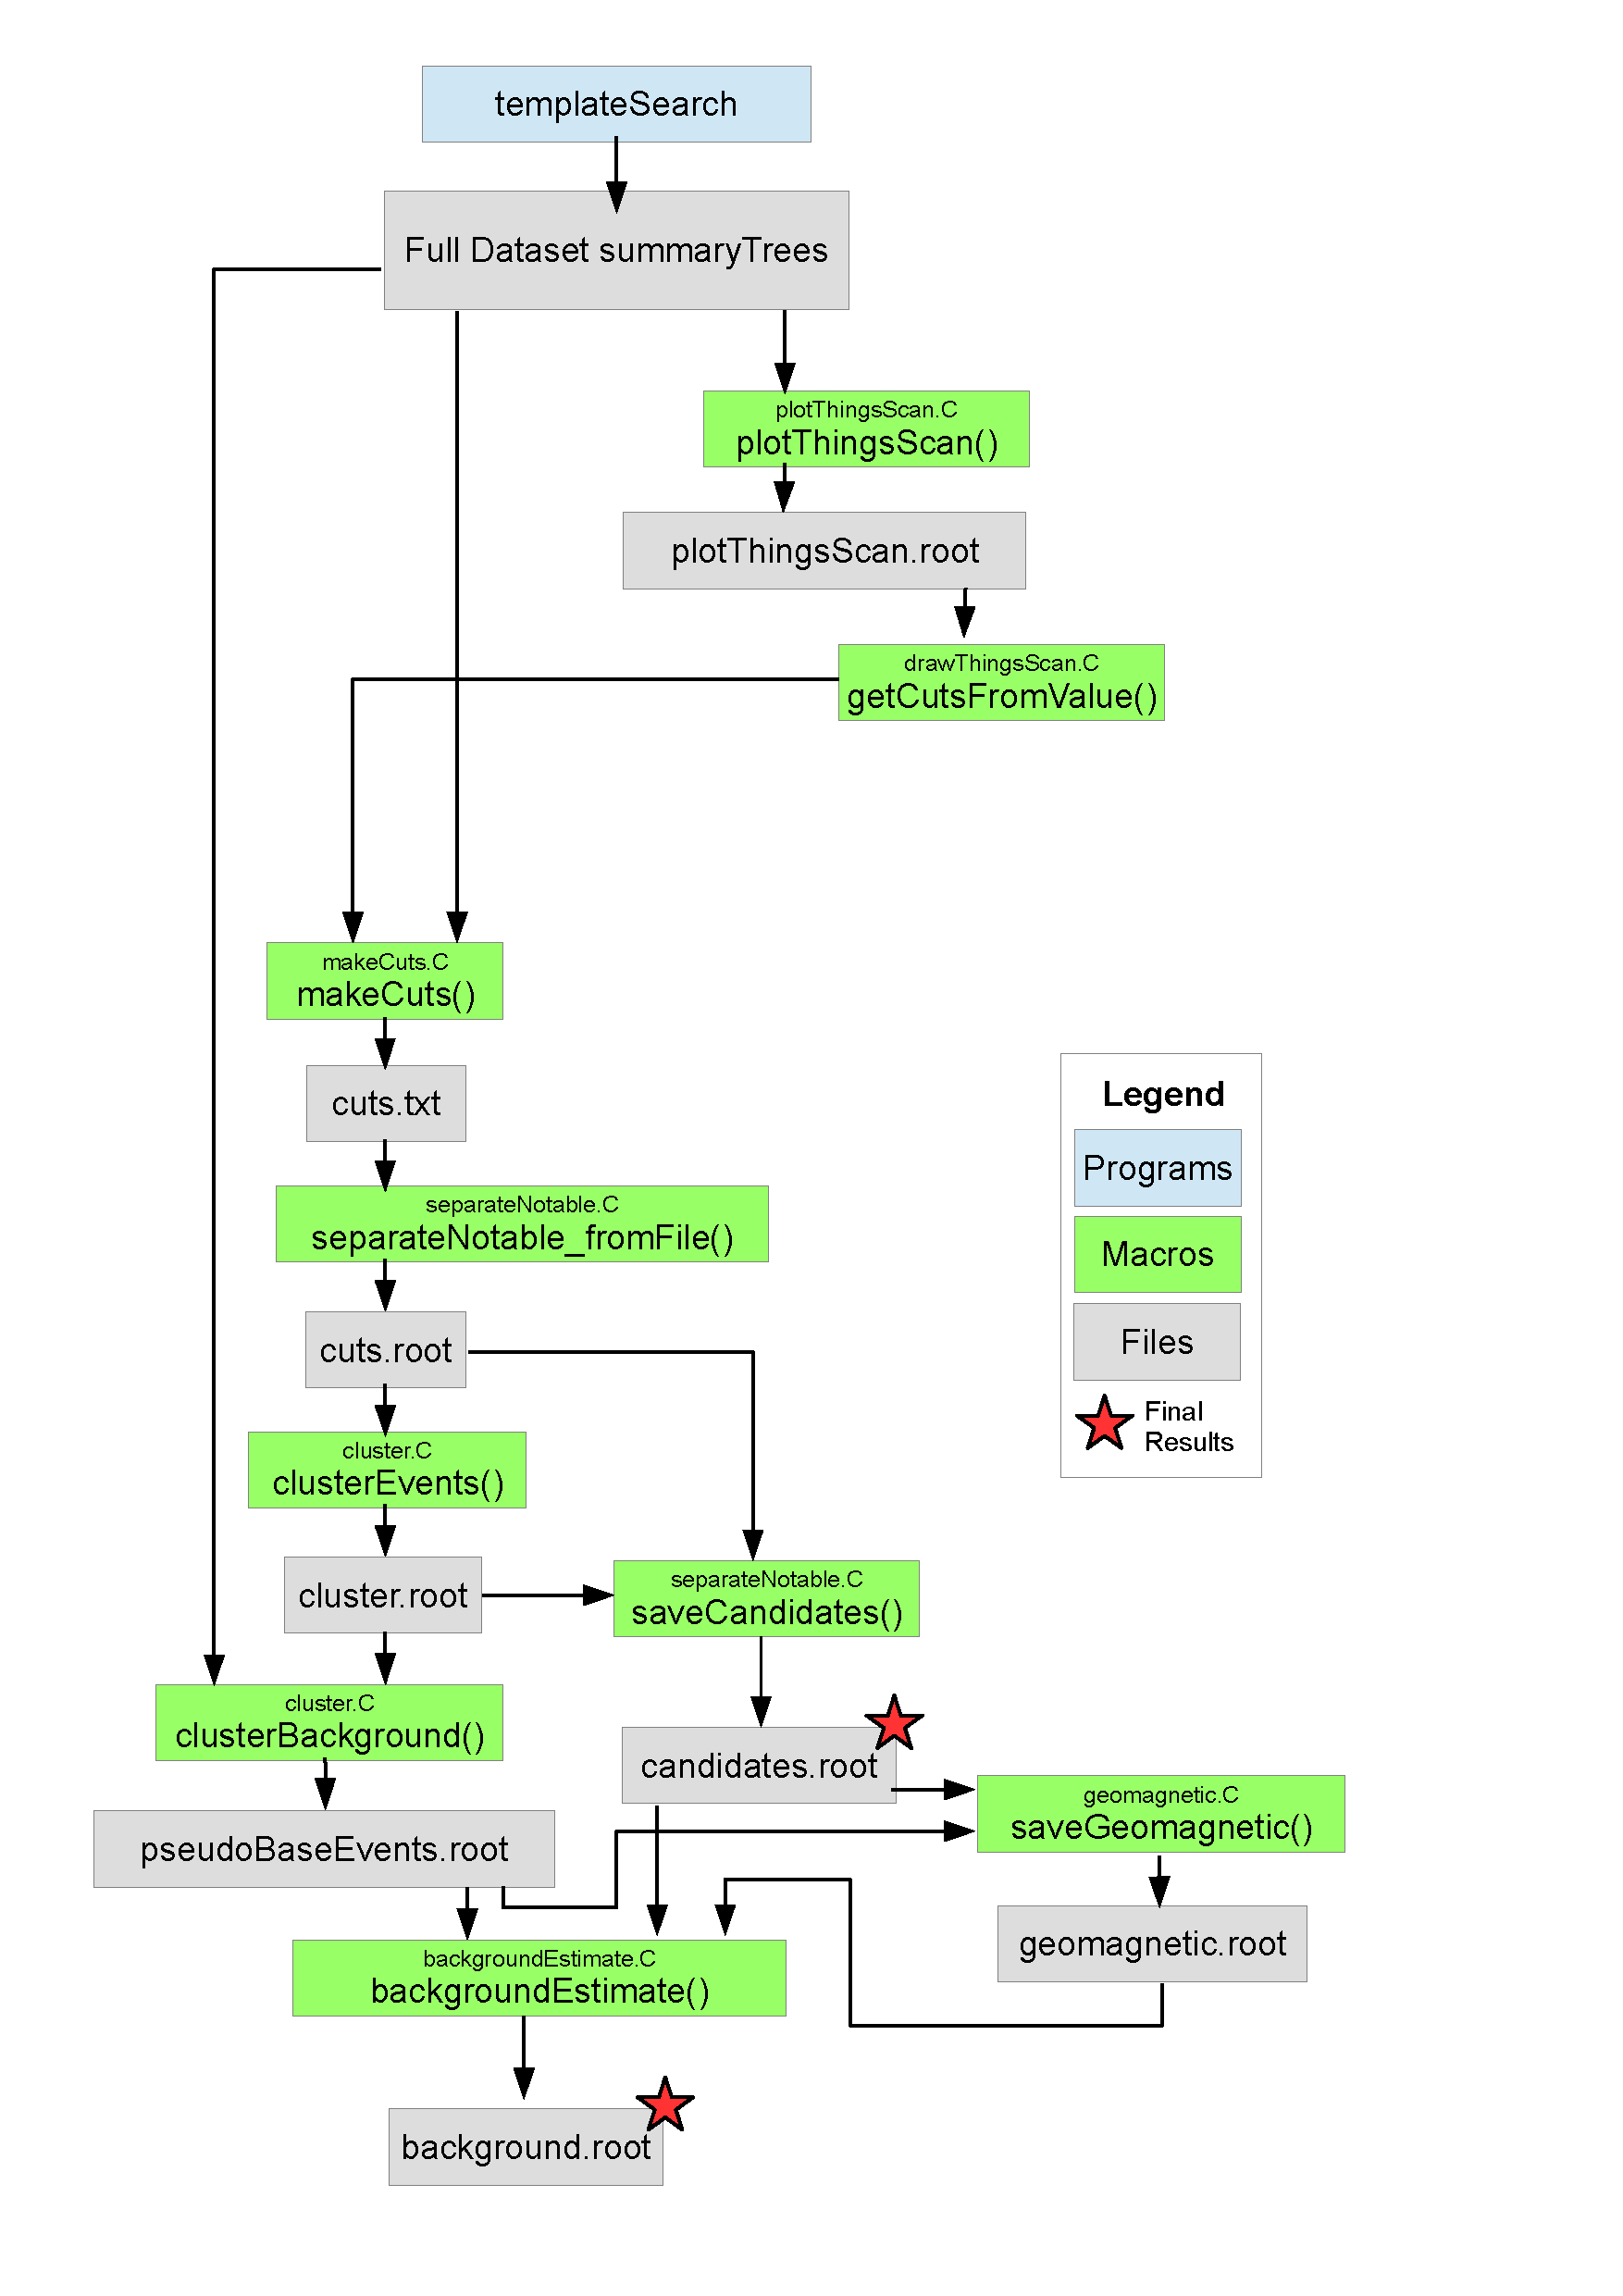
\includegraphics[height=0.8\textheight]{figures/AnalysisDiagram}
	\caption{A diagram depicting the order in which analysis steps are taken, the intermediate storage files saved to disk, and the function names and ROOT macros where the code is located.  These steps are described in detail throughout this chapter.  The storage locations of final results are noted with red stars.}
\end{figure}	
		
%	The data recorded by the ANITAIII flight instrument requires a significant analysis effort to extract a meaningful physics result.  Using the raw digital values recorded from each channel, we can establish the analog electromagnetic environment surrounding the payload during brief moments the trigger system determined a physics event may be occurring.  From this, we can use an  understanding of the physical geometry of the antennas mounted on the payload, including their orientation and electrical responses, to determine the cause of any incident wave patterns read out by the digitizers.  Once these wave patterns are identified and classified, they can be sorted into signal and noise, background thermal or anthropogenic, via a series of procedural cuts.  This section details the process and results of this analysis.
	

\section{Software Package Overview}
	The analysis was done with a variety of software packages created by the ANITA collaboration.  The relevant packages used in the analysis described in this thesis are described in the following section.  The range from tools for interfacing with , to ANITA specific calibration and interferometric mapping, to this-thesis specific packages for template correlation, clustering, and background estimation.  The packages are described in order of dependency, with most independent packages listed first.
	
	The cosmic ray search was done primarily in C++ using libraries from the ROOT Data Analysis Framework~\cite{ROOT}.  ROOT, developed at CERN, provides a variety of data storage objects and plotting functions optimized for physics experiments.

	\subsection{ROOT FFTW interface: libRootFftwWrapper}
		Fourier transforms were done using the the Fastest Fourier Transform in the West (FFTW) package.  This package is not designed to be used with the ROOT objects that the remainder of the packages are based around, and so an interface library, named libRootFftwWrapper is used~\cite{libRootFftwWrapper}.  This package not only provides an interface however, it also includes a large number of ANITA related numerical recipes.

	\subsection{Event Reader Software: eventReaderRoot}
		The data taken by the ANITAIII instrument is written in a compressed c++ binary class format to disk.  This data format requires minimal computational load and very fast write speeds, with minimal storage space overhead.  This data format requires a standardized class structure that is stored in the eventReaderRoot code library~\cite{eventReaderRoot} in order to accurately read and extract any values.  The raw data taken in flight is converted to ROOT objects, which increases data read speed and enforces data quality, with the tradeoff of slightly increased storage space and a one time computationally complex conversion.  The eventReaderRoot library also stores information about each flight, such as the number of antennas and their mapping to RF channel, as well as tools for applying the calibration constants to waveforms.

	\subsection{Coordinated Analysis Framework: AnitaAnalysisFramework}
		In order to facilitate active collaboration between multiple analyzers, much of the analysis software was consolidated into a library named the Anita Analysis Framework~\cite{anitaAnalysisFramework}.  It provides a standardized set of C++ classes for storing and calibrating digitized LABRADOR waveforms in memory, implementing filtering algorithms, implementing agreed-upon common analysis tools, and a shared output format.
		
		This framework, most importantly, provides a C++ summary class with agreed upon reduced quantity values of interest.  This object, named the AnitaEventSummary, is created for each event taken during the flight, and is designed to be filled by any analysis routine with all values required to do a full physics analysis of the flight data.  This prevents computationally burdensome calculations used in calibration and interferometry from being repeated multiple times.
				
				%crab
	\subsection{University of Chicago Event Analyzer: UCorrelator}
		The data taken by the ANITA instrument requires processing to be useful in a physics analysis, and many of the computational techniques can be shared across multiple analyses.  For this analysis, I have used and collaborated to the UCorrelator software packaged developed primarily by Cosmin Deaconu at the University of Chicago~\cite{UCorrelator}.  With the addition of my own bug-testing and feature expansion, this package has been used to do the base-level numerical computations for this analysis.
		
		
	\subsection{Event Display: anitaMagicDisplay}
		The anitaMagicDisplay package \cite{anitaMagicDisplay} allows a user to quickly and easily display many of the most relevant raw and reduced data values for any event in the flight.  The package provides a Graphical User Interface (GUI) that can simultaneously display waveforms captured from the entire instrument sorted in various ways.  It also include dynamically selectable filtering strategies, maps and summaries of multiple interferometric reconstruction techniques, and payload orientation information.  
		
	\subsection{Miscellaneous utility functions: anitaEventCorrelator}
		A separate library that includes some additional important functionality is anitaEventCorrelator~\cite{anitaEventCorrelator}.  The most important class in this code is UsefulAdu5Pat, which takes raw GPS sensor information, as well as Earth geometry and Antarctic topographical information, and provides a method for mapping spherical payload coordiates to a point on the continent, and vice-versa.
		
		
	\subsection{Thesis analysis specific: benCode}
		The eclectic accumulation of code used in this analysis is stored in a variety of libraries, macros, and compiled programs collectively named benCode~\cite{benCode}.  Though there are many offshoot routines for debugging and the determination of specific values of interest, the main path for the analysis is summarized in Figure \ref{fig:AnalysisDiagram}.

	
	
	
\section{Dataset and Blinding Procedure}
	The ANITAIII flight took Avoiding the introduction of bias into the resulting measurement through the subconsious desires of the analyzer is a constant struggle.  Several techniques have been employed to minimize this insidious bias.
	
	\subsection{Dataset for analysis}
		The ANITAIII instrument was put into flight configuration on December 9th 2014, which marks the beginning of the run numbering.  However, due to non-optimal launch conditions, the payload was not launched for another week.  During this time, the system remained on, taking data at a reduced rate for last minute data validation and bug fixes.  The successful launch on December 17th 2014 at 19:23 UTC is shown in Figure \ref{fig:AnitaLaunchAltitude}.  The pre-amplifiers were turned on midway through the ascent in order to protect them from the high powered anthropogenic noise at the launch facility. Run 130 is the first run at altitude with all systems operating in final flight configuration.  Run 439 was the final run recorded to disk before the instrument was powered down for descent.  The final event was taken on January 9th 2015 at 05:52 UTC.
			
\begin{figure}
	\label{fig:AnitaLaunchAltitude}
	\centering
	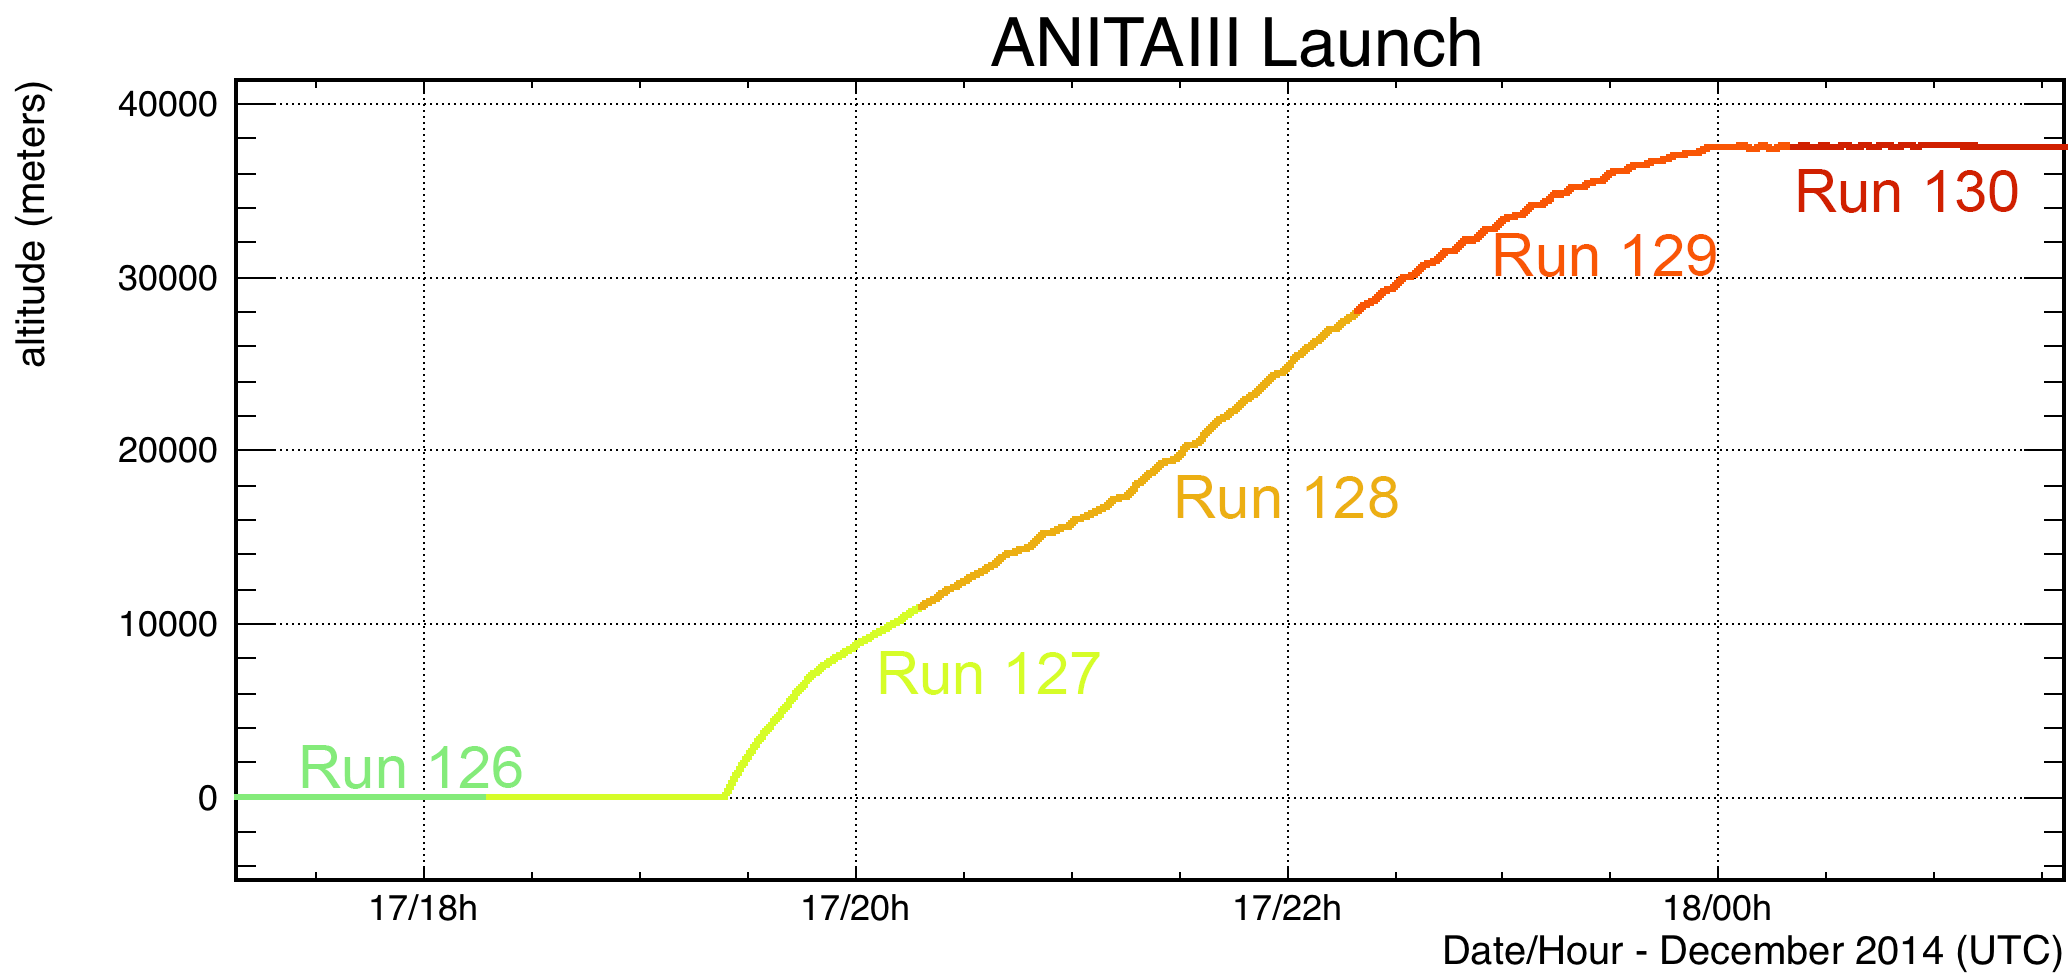
\includegraphics[width=\textwidth]{figures/LaunchAltitude}
	\caption{Altitude data captured by the on board GPS on launch day.  Colors refer to the run number of that data.  Run 130 is the first run where the instrument was in full data-taking configuration and at float altitude.}
\end{figure}	

		During the 22 days and 10 hours of active data collection at altitude, between run 130 and run 439, ANITAIII captured 78,630,542 events.  Runs 257 through 263 contain no data due to a bug in the Prioritizer daemon causing the Ramdisk to fill, and preventing the acquisition software from recording events.  This outage occurred on Christmas day, and resulted in an 11 hour data blackout, from December 25th at 17:13 to December 26th at 04:28.
		
		For the cosmic ray analysis, only events that fired the horizontally polarized L3 trigger are considered. The geomagnetic radiation that is predicted to dominate the electromagnetic emission of an EAS is expected to be mostly horizontally polzarised. 40,098,640 events fall into this dataset.  77,336 events fired both the horizontal and vertical L3 trigger, however they are not treated in any unique manner.
		
		Additionally, the payload initialized a digitization twice per second regardless of the RF trigger, once initiated by the GPS second and once initiated by the CPU.  There were 839,762 of these ``minimum bias'' events recorded during the flight.  These events are also processed and used to determine the background noise environment during the flight.
		
	
	\subsection{Philosophical reasoning For blinding and past methods}
		Much discussion took place within the collaboration in order to prevent unwanted analyzer bias from being a significant effect of any analysis result.  Unconscious bias is an inherently human trait, the cold unfeeling rules of nature do not bend to the whims of our emotions or desires.  However, by allowing analyzers to pick and choose methods and procedures and cuts, it is possible that a result may unwittingly reflect those same desires and emotions.  For example, an ambitious physicist, who desires to further his career, may see the opportunity to do so through an exciting and controversial result that makes other scientists take note of his work.  On the other extreme, an exhausted physicist, who does not want to defend a controversial result, could ``play it safe'' and tune his analysis to find a result in agreement with other experiments.  Both these biases are undesirable, but both could be subtly effecting results though no fault of either scientist.
		
		The solution to this problem is to introduce a method in which the result is entirely outside of the experimenters control until all analysis procedures are complete.  In previous ANITA analyses, this was accomplished by ``hiding'' 90\% of the signal data, only allowing analyzers to use a 10\% fraction of the full set to tune their cuts.  Once the cuts were set to meet a desired background rejection fraction, the reminder of the events that did \textit{not} meet the cut requirements would be revealed.  A statistical method, known as the ABCD method, could be used to estimate the number of background events within the signal box from purely random statistical fluctuations.  Any number of events in excess of this background estimate would then be considered signal.  This method had several drawbacks. First, an inability to determine signal from background on an event by event basis leaves a possibility that the most interesting events are background.  Additionally, it allow anthropogenic background to escape observation within the 10\% data set, requiring it to be removed manually by hand later, re-introducing bias.
		
	\subsection{ANITAIII CR blinding technique}
		For the ANITAIII CR search, it was decided that a 10\% - 90\% blinding requirement was unnecessary.  The energy spectrum and flux density of CRs are measured well up to the UHE range.  Additionally, both ANITAI and radio extension projects at terrestrial cosmic ray observatories have measured the radio EAS signature of a CR interaction with the atmosphere.  The ANITAIII results have also been subject to a fully blind analysis previously in a neutrino search that reported 4 transient events matching signal.  For this reason, a novel and more lax blinding procedure was agreed to for this earch.

		The signal of greatest interest in this analysis is a regenerated tau neutrino transiting through the earth and hadronically decaying in the atmosphere.  Though the primary particle is different from a CR EAS, the shower will evolve in a similar fashion and produce a similar radio pulse.  The defining characteristic of this signal is a polarity with the same sign as a direct EAS shower observation, but with an incidence angle below the horizon (beyond misreconstruction uncertainty).  To prevent any bias in this signal channel, the polarity of all events has been randomly inverted.  This will create a random distribution of polarities, and prevent an analyzer from determining whether any particular event is of interest.
		
		Additionally, only signals that triggered the horizontally polarized L2 trigger are analyzed to preserve the integrity of the neutrino search.  Observations of CR EAS signals are expected to be primarily horizontally polarized, while in-ice neutrino interactions are expected to have primarily vertically polarized observed signals.  This also helps to reduced the computational workload, as each polarization trigger accounted for approximately half of the overall events.
		
			
\section{Event Quality Cuts}
	Events taken with the ANITA instrument must first pass basic checks on their quality.  ANITAIII does not seem to suffer from significant issues related to the digitization or storage of waveforms, however there are several observed bad event types that can be identified and removed prior to analysis.

	\subsection{Payload Blasts}
		The ANITAIII flight was plagued by high power signals that seem to emanate from the payload.  These events, called payload blasts, have a large amplitude signal in several neighboring phi sectors and tend to happen in rapid succession.  A sample payload blast event can be seen in Figure \ref{fig:payloadBlast}.  The blasts characteristically have high total RF power in the bottom two rings of antennas, but very little signal power in the top ring, suggesting that these events have a source on-board the payload.  Blasts also do not have high interferometric peaks, adding further evidence that they are spherically propagating electromagnetic waves with a source on the payload, and suggesting that they will likely be removed through signal cuts later in the analysis process.
		
		The primary metric used to select and remove these events is this ratio of total waveform power between top and bottom rings (Equation \ref{eqn:topToBottom}). This distribution can be seen in Figure \ref{fig:payloadBlastDist}.  The cut for these events was placed at a value of 3, which eliminates approximately 731k  events (1.77\%) of events from the Hpol data set, while effecting a trivial number of non-RF triggered thermal events.  The source of these blasts is unknown, though there is much speculation to their cause, and were present in both the ANITAI and ANITAII flights.  Removing these events from the dataset is done prior to all other analysis steps.  
		
\begin{equation}
	\label{eqn:topToBottom}
	R_{topToBottom} = \cfrac{\sum\limits_{n=0}^{N} V^{2}_{bottom}}{\sum\limits_{n=0}^{N} V^{2}_{top}}
\end{equation}
		
\begin{figure}
	\label{fig:payloadBlast}
	\centering
	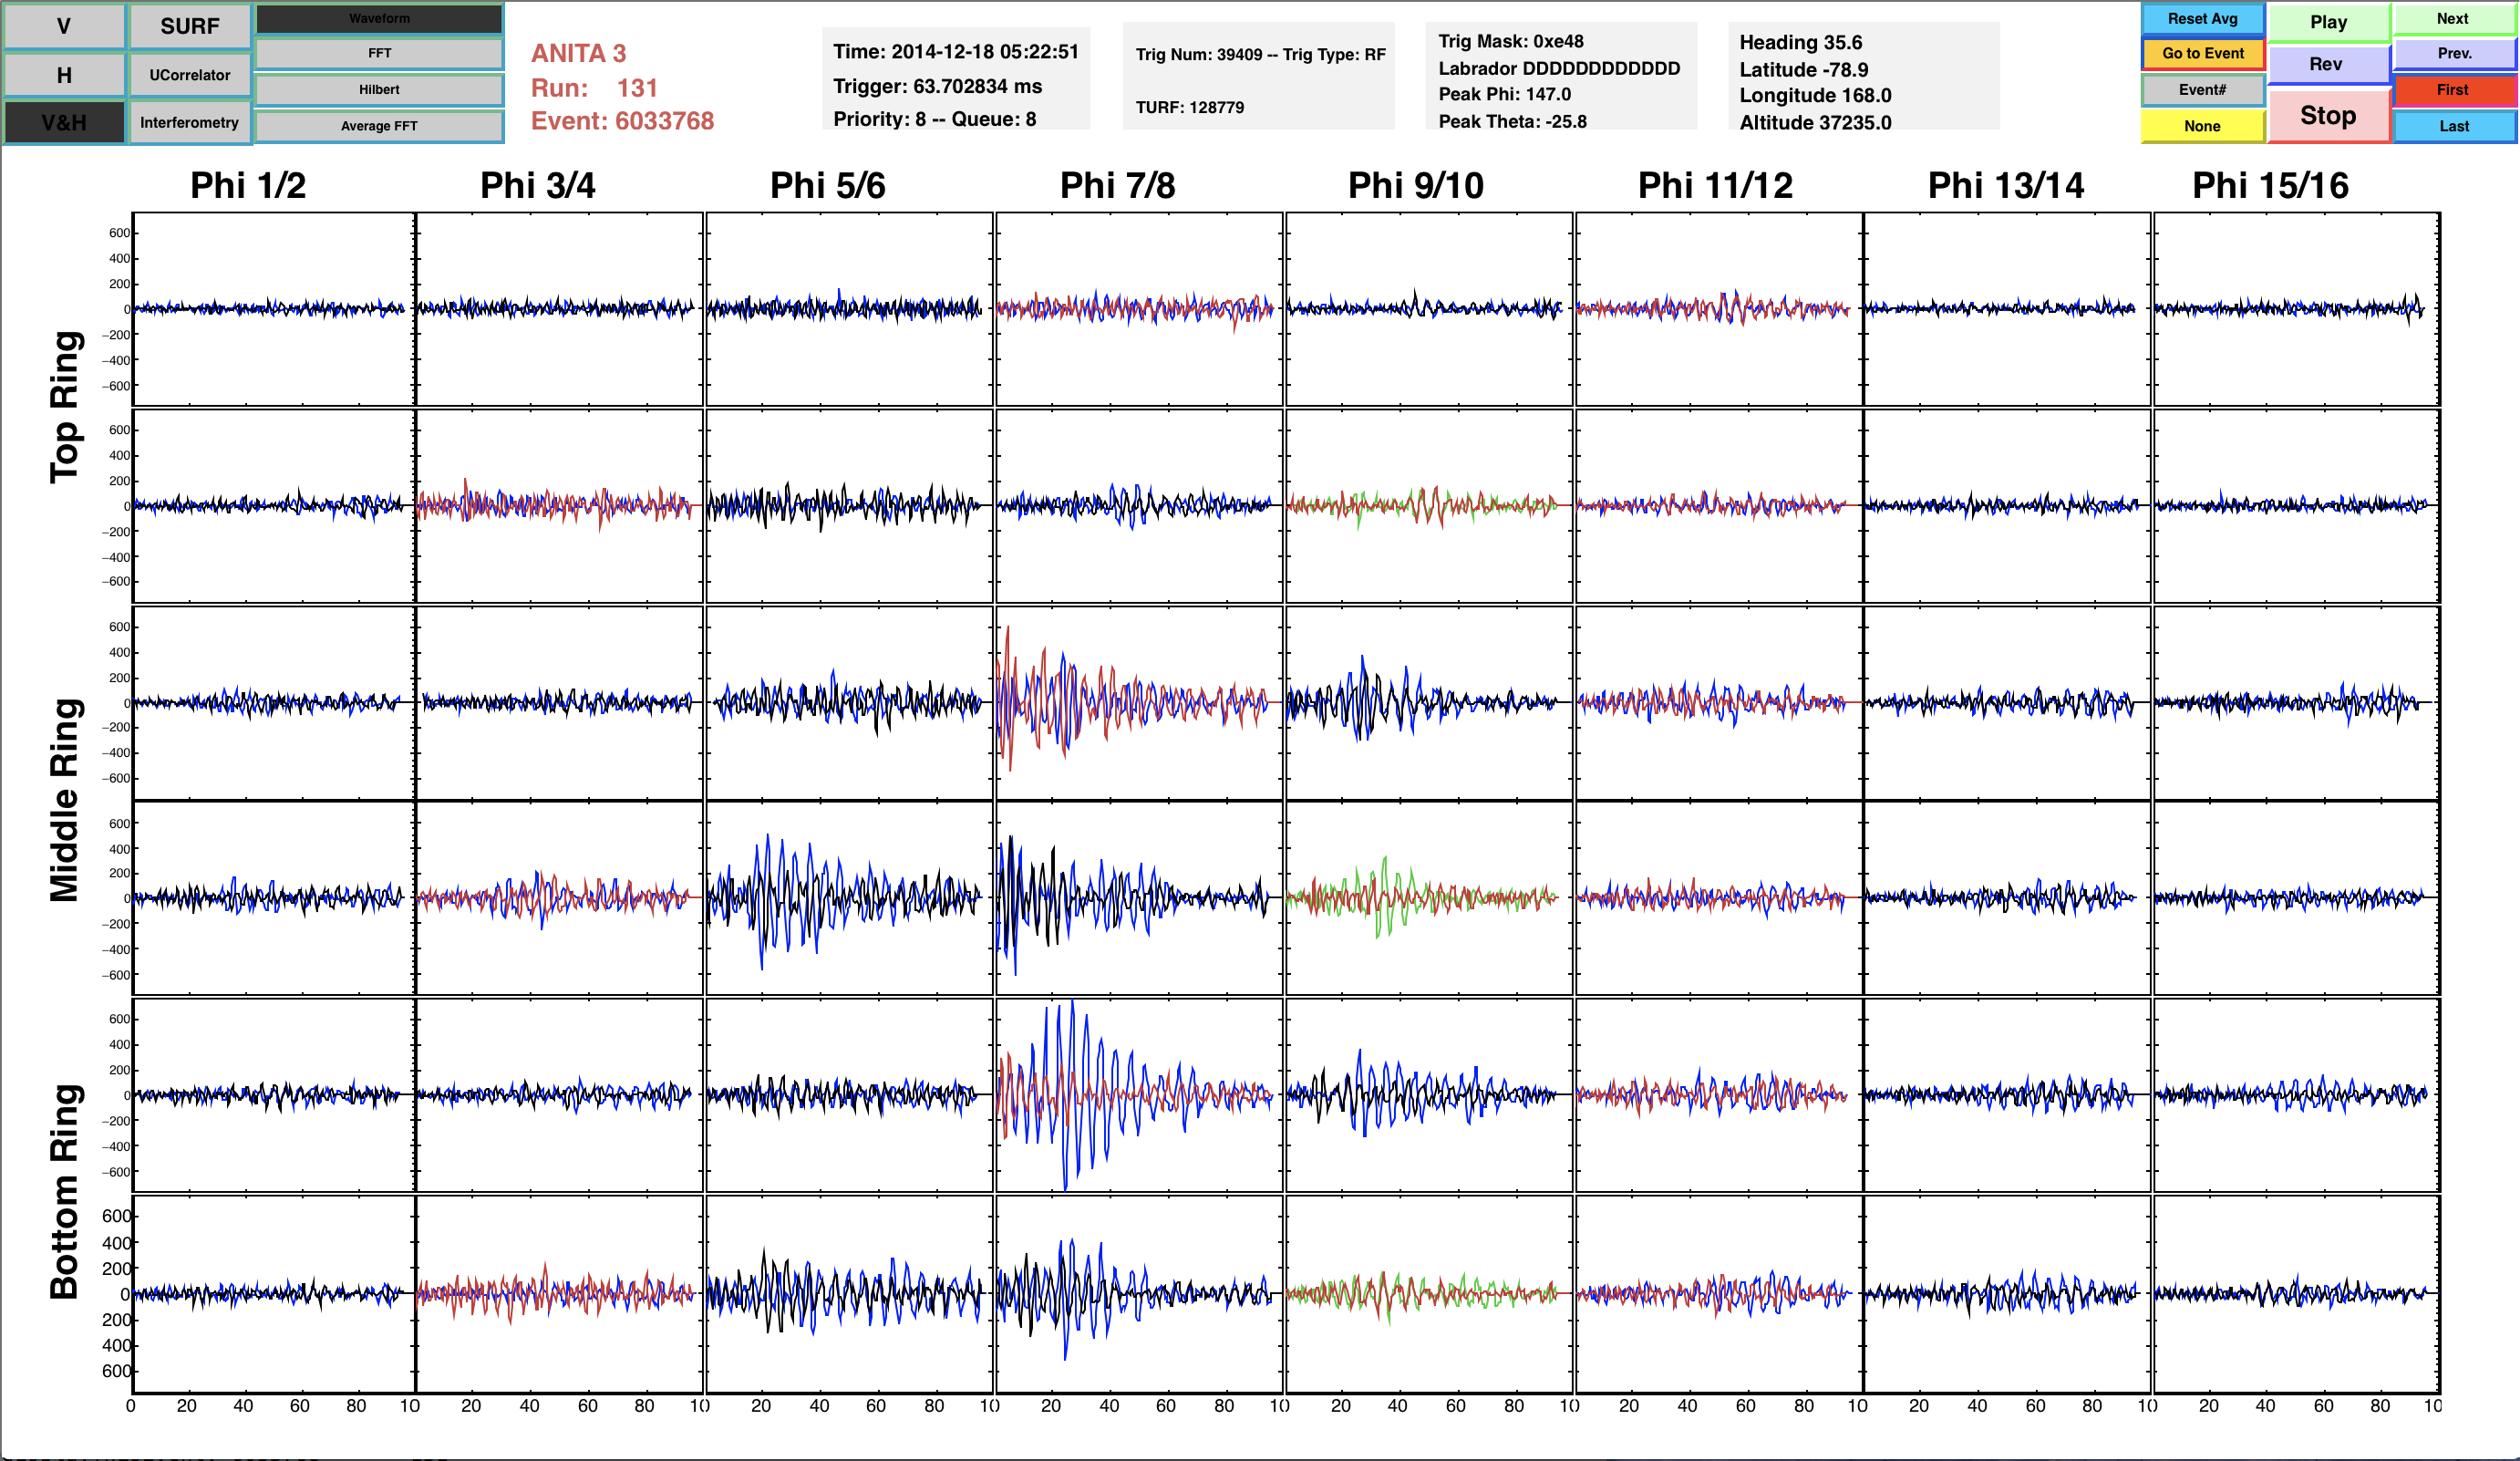
\includegraphics[height=0.5\textheight]{figures/payloadBlast}
	\caption{A magicDisplay screen capture of a suspected payload blast event.  This event was selected due to the high ratio of power between the top and bottom antenna, 6.15 for this particular event.  This pulse is additionally part of a 14 event train of pulses}
\end{figure}

\begin{figure}
	\label{fig:payloadBlastDist}
	\centering
	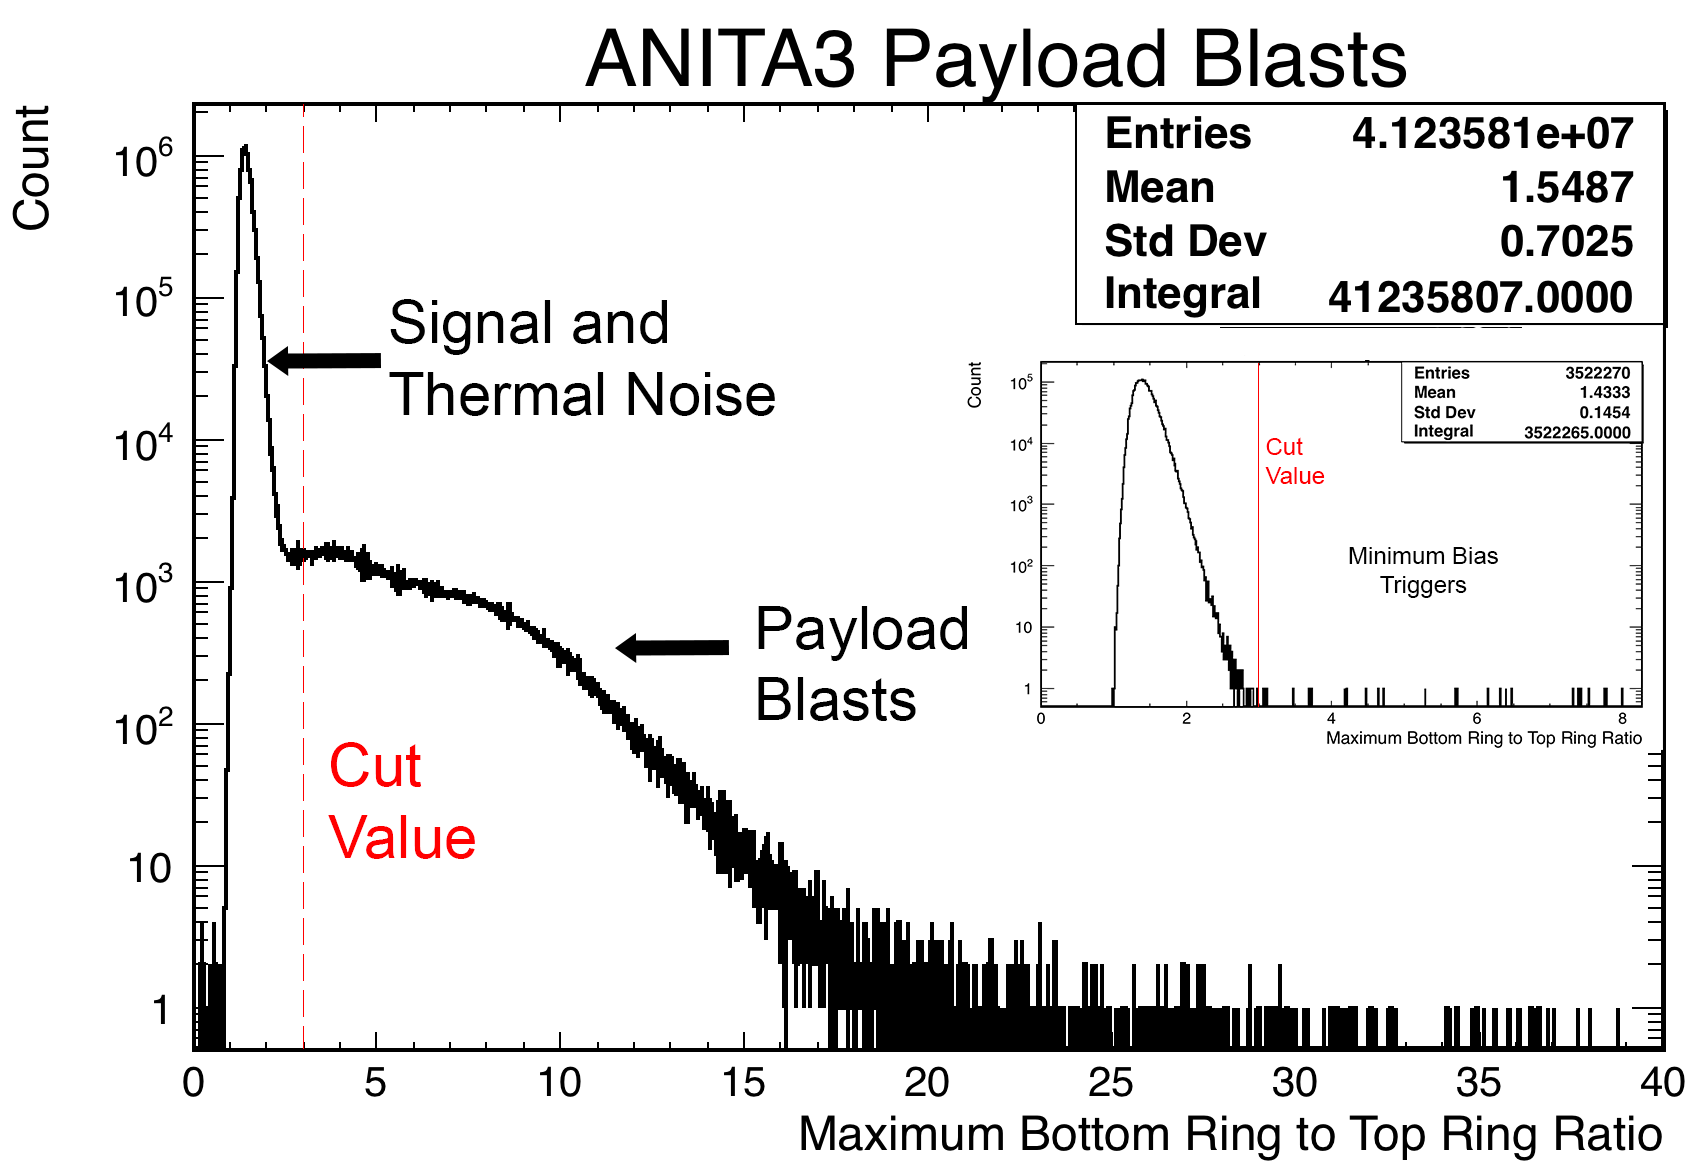
\includegraphics[height=0.5\textheight]{figures/payloadBlastDistribution}
	\caption{The event distribution of the ratio between the power measured in top and bottom rings of antenna for all horizontal polarization triggered phi sectors.  The distribution for non-RF triggered events is displayed as well, within the full distribution plot.  Red dashed lines denote the location of the quality cut.}
\end{figure}
	
	\subsection{SURF Saturation}
		A small fraction of events have recorded voltage values outside the dynamic range of the LABRADOR digitizer.  Though several of these are from extremely high power sources within the field of view, several saturation events are caused by single bit errors in LABRADOR digitization.  These have the characteristic of having a single point a power of two higher than the remaining points in a waveform.  For simplicity, all events with these bit errors are excluded.
		
\section{Digital filtering}
	The stored digital waveforms can be improved by the removal of well understood background signals.  Anthropogenic digital communications often take the form of circularly polarized constant wave (CW) sources, and are present superimposed in much of the data.  Their sources include both manned and unmanned bases distributed throughout the continent, as well as orbiting satellites visible above the horizon.  These CW signals have a significant effect on both the trigger circuit and the post-flight analysis of digitized data. A spectrogram of a period of the flight can be seen in Figure \ref{fig:spectrogram}, with the CW peaks from satellite noise clearly visible at 220MHz and 380MHz.

\begin{figure}
	\label{fig:spectrogram}
	\centering
	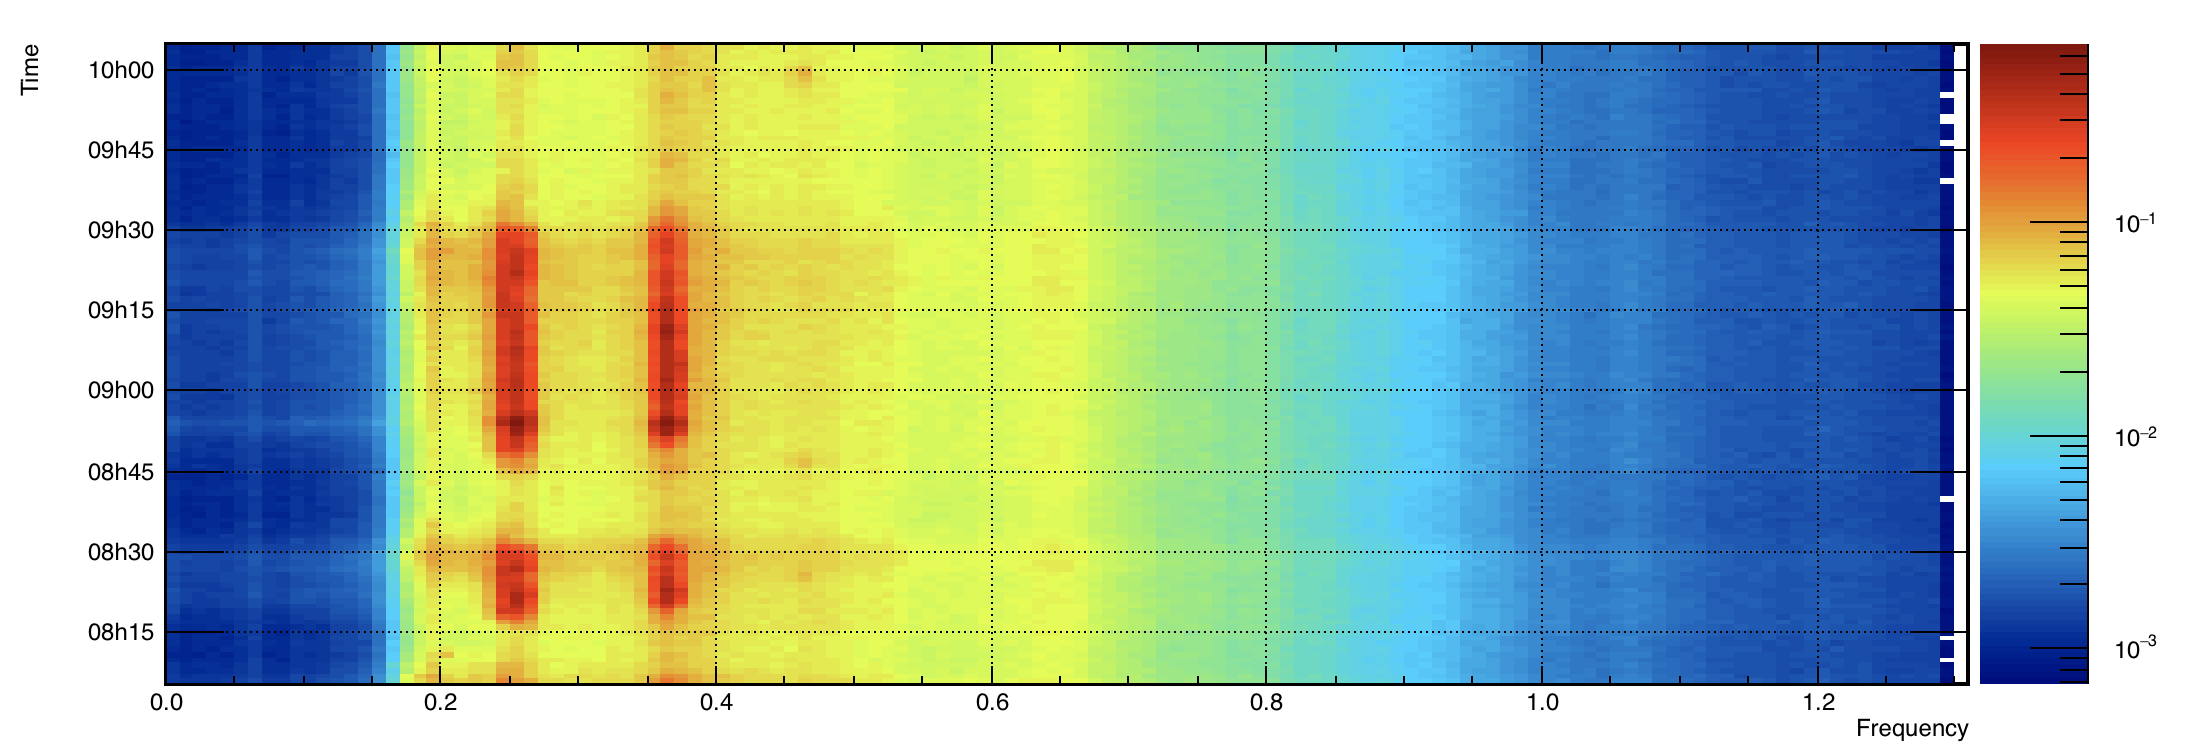
\includegraphics[width=\textwidth]{figures/spectrogram}
	\caption{A spectrogram of the measured RF signal from a single antenna pointed north during the beginning of run 371.  The Z-axis is linear power.  The red regions at 220MHz and 380MHz are frequency bands with high power due to orbiting satellites.} 
\end{figure}

	The effect these CW signals have on the trigger is twofold.  Firstly, they compress the tunnel diode by increasing the total power of the input signal, pushing the diode response out of its square-law range.  Additionally, CW sources force an increase in the threshold voltage used on the comparator circuit used to trigger on the signals in order to maintain an acceptable global trigger rate.  In many cases, the amount of power from CW sources forces mulitple phi sectors to self-mask, as no DAC threshold setting can appropriately limit the L2 trigger rates from a specific phi sector.  These negative effects cause a decrease in the sensitivity of the instrument to physics events with low signal power, and decrease the overall instrumented volume.  For the ANITAIV flight, a programmable analog notch filter board was flown to eliminate these effects, designed using the known CW frequencies observed in the ANITAIII flight.

	
	Despite these two effects, impulsive candidate signals can still be measured while superimposed on the CW source.  In these cases, the CW causes the interferometric image to be ``pulled'' towards the source of the signal while also presenting false peaks in the image.  To remediate the effects of these signals on the pointing and post-flight analysis, we can apply a digital filter that removes specific frequency bands.
	
	
	\subsection{Sine Subtraction Filtering}
		The filtering technique used in this analysis has been dubbed sine-wave subtraction.  Digital Finite Impulse Response (FIR) filters introduce dispersion, which will negatively effect the reconstruction accuracy and final SNR of any incident physics signal.  To alleviate this, a method was developed which involves procedurally fitting the phase, amplitude, and frequency of a sine wave to each waveform, then subtracting that sine wave from the signal.  This is repeated iteratively until the resulting subtracted wave does not have a large fractional power decrease.  This acts to remove single frequency bands from each channel without adding a significant amount of dispersion, nor diminishing physics signal or thermal noise power.  The drawback of this method is that it requires multiple fits per waveform, which is computationally expensive.  The computations for this filtering strategy takes approximately half of the total computation time.  The framework and coding of the SineSubtract algorithm was done by Cosmin Deaconu.  

	The sine subtraction works by iteratively fitting a sine wave to each captured waveform individually, minimizing on the amplitude, phase, and frequency.   To aid in computational efficiency, the range of frequencies and amplitudes that the fit could minimize over were adaptively altered based on a previously generated full flight frequency spectrogram.  This adaptive component has a configurable ``exponent'' variable that controls how strictly   This best-fit function is then subtracted from the waveform, yielding data with a single frequency component removed.  This process is repeated until the ratio of the power subtracted from the waveform over the total power in the original waveform is below some configurable threshold a specified sequential number of times.  For this analysis, a ratio of 0.1 was used, and 3 failed iterations were allowed.  The key used to generate this filter in the AnitaAnalysisFramework is ``sinsub\_10\_3\_ad\_2''.  
	
	An example of the effect that the filtering has on a calibration pulser can be seen in Figure \ref{fig:SineSubtractMaps}.
	
\begin{figure}
	\label{fig:SineSubtractMaps}
	\centering
	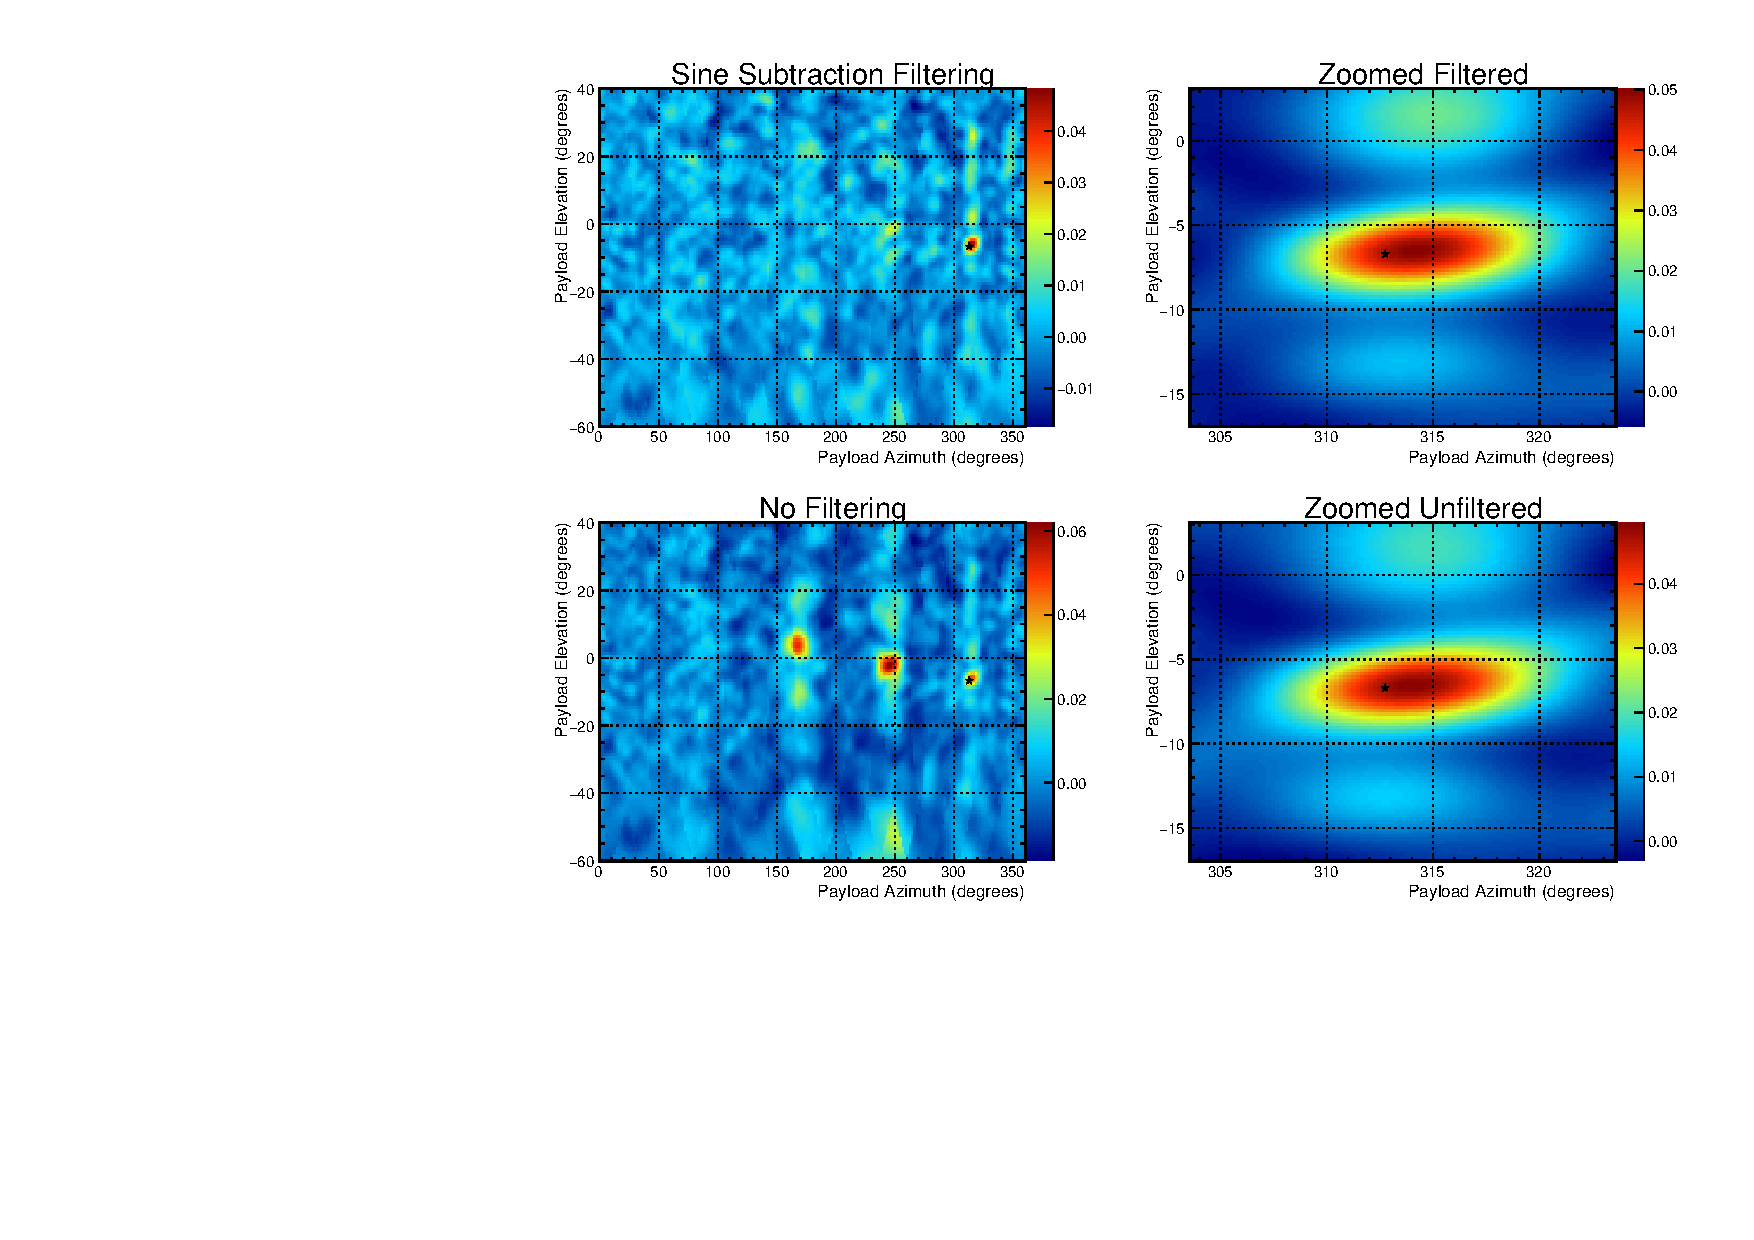
\includegraphics[height=0.5\textheight]{figures/SineSubtractMaps}
	\caption{The effect that sine subtraction filtering has on interferometric mapping.  This particular event, 56765803, is a WAIS pulser event.  35.9\% of the initial power was removed in the filtering process.  Without filtering on this event, the peak of the interferometric map is not pointed at WAIS divide (denoted by the black star).} 
\end{figure}

\section{Waveform Reconstruction}
	To extrapolate the measured signal on the ANITA instrument back to a physics signal or background noise event, we must combine the various waveforms captured around the instrument.  By summing the values various waveforms with specifically determined time offsets, it is possible to determine the level of coherence of the electromagnetic environment.  Once an arrival direction is determined it is possible to reconstruct the signal, averaging out the random thermal and electronic noise.
	
	By correlating the waveforms captured between various antenna pairs it is possible to establish time delays in which multiple channels maximally constructively interfere.  Known as interferometry, a radio astronomy technique, it makes use of the known physical separation vector between the antennas and the propagation delay for any incident plane wave.  generate a map of likely pointing directions.  ANITA has three vertical tiers of antennas, each separated from each other, and at least three co-pointing phi sectors that are expected to observe events from any angle.  Using the combined baseline offsets from these antennas, it is possible to overlay 9 different interferometric maps to create a pointing map.  By finding the peak of this map, a vector pointing away from the payload can be traced to the ice, where a map of the vertical height of the continent can be used to create a map of events on the ground.
	
	\subsection{Radio Interferometric Mapping}
		Interferometric mapping is a method developed to compare measured time domain waveforms captured by antennas with a physical baseline offset with the goal of determining likely incoming plane wave direction.  This is accomplished by calculating the timing offsets expected from each direction of a pair of antennas in elevation and azimuth, computing the correlation function of the two waveforms, then weighting each direction in relation to the correlation value at that specific timing offset.  An example of a map created with a single baseline pair is seen in Figure \ref{fig:singleBaselineCorrMap}.  With multiple baseline pairs, each with a different distance vector angle between them, one can overlay multiple correlation maps to determine a most likely incoming plane wave direction.
		
		
	\subsection{Coherent Waveform Sum}
		The electronic and thermal noise present in each channel limits the sensitivity of the instrument to EAS signals with low power.  Since the power within the radiation of an EAS shower varies linearly with the energy of the particle, low energy showers, which have a higher flux rate, will have signal to noise ratios approaching one.  Additionally, polarization information and frequency content are effected by any noise present in the system.  Averaging waveforms from multiple channels will reduce this incoherent background noise by a factor of $\frac{1}{\sqrt{N}}$.  After determining the peak interferometric pointing direction, it is possible to align the channels that received signal from an incident radiation field and average them together.  An example of this is shown in Figure \ref{fig:coherentSum}.
	
	
	\subsection{Ray Tracing to Continent (with index of refraction)}
		Another tool made possible through interferometric mapping is that it allows us to point a captured event back to its incoming direction, determining the likely incident cosmic ray interaction location.  Ultimately, it would be most interesting to point an incoming particle back to a location on the sky for statistical source determination.  Additionally, it is important to determine whether a measured event came from a particle physics interaction, or was merely an anthropogenic background noise impulse.  By developing a base list from USAP and other international Antarctic programs, we can determine whether a specific event points back to a known base.
		
	\begin{equation}
		\theta_{horiz} = ArcCos(\cfrac{R_{e}}{R_{e}+H})
		\label{eqn:thetaHoriz}
	\end{equation}
	Where $R_{e}$ is the radius of the earth, and $H$ is the altitude of the payload
	
	\subsection{Immediate Pointing Cuts}
		Real physics signals have a small range of elevation angles where their detection is most likely.  The highest probability incident direction for an EAS is near the horizon, however noise events will point more evenly in all directions.  Using this knowledge, we can cut out events that have very steep elevations.  A distribution of event pointing direction can be seen in Figure \ref{fig:elevationAngle}.


\section{De-dispersion}
	The antenna, filters, cables, and amplifiers are responsible for introducing a frequency dependent gain and group delay to the observed signals.  These elements act to disperse the power in the signal across tens of nanoseconds from what was emitted from the relativistic shower at the critical angle as a highly impulsive, picosecond length essential delta-function like electromagnetic field transient.  The impulse response, or complex phasor representation of this dispersive effect, was measured for the signal chain immediately preceding the flight for each of the 96 channels, and for all 48 antennas in a controlled manner in Palestine the summer beforehand.  These two effects are then combined and used to determine a whole system impulse response that relates the measured ADC values at the LABRADOR digitizer to an electric field incident at the payload.  By reversing the dispersive process, via Weiner deconvolution (described below), we can both increase the instantaneous power of a signal and compare it directly to the electric field radiation output of high energy particle shower simulations such as COREAS or ZHAires.
	\subsection{Generation of transfer function}
		The transfer function of the system was painstakingly developed and utilized a variety of both time domain and Fourier transformed frequency domain manipulations.  These each introduce their own errors, as many of them require assumptions about the incoming signal.  I'll detail the full process of generating the transfer function in an appendix.
	\subsection{Signal to noise ratio of impulse response}
		Any band limited deconvolution process requires a knowledge of the signal to noise ratio of the transfer function as a function of frequency (SNR(f)).  Since the transfer function merely relays the amplitude and phase differences between an input and output signal (represented in either a complex phasor or a time domain waveform), one must also have an understanding of the total power contained within the input and output signals.  If, for example, both the input and output signal contained very little power out of a specified band pass, it could be wrongly assumed from a transfer function that the signal chain was able to pass frequencies that are out of the band pass.
		The "signal" and "noise" of this must therefore be defined, as the spectral power has multiple sources.  The principle   
	\subsection{All-Pass Deconvolution}
		The impulse response used to deconvolve waveforms has been colloquially named the All-Pass deconvolution method.  An ideal deconvolution, one that uses both phase and amplitude information to remove the instrument response, is poorly defined outside the instrument bandwidth.  Since the instrument blocks any signal outside this frequency range, reversing the procedure introduces what is in essence a "divide by zero" error that grossly amplifies signal power outside the band.  The simplest way to avoid this is to disgard the frequency dependent amplitude information, and only correct for the phase.  Due to the relatively flat spectral response of the ANITA system, this is a good first approximation.  The resulting waveform "stacks" signal power from all in-band frequencies on top of one another, increasing the observed peak to peak signal to noise ratio and offering a larger separation between signal and noise events during analysis cuts.



\section{Template Correlation}
	Though any physics experiment that aims to separate background events from signal events requires a general understanding of characteristics inherent to either group, measurements and simulations of UHECR induced EAS signatures provide a waveform template that can be used to strongly cut on signal events.  The simplest assumption, that an EAS will produce a broad spectrum, short duration, electromagnetic pulse, drives both the overall design of the payload, as well as several of the analysis cuts.  Determining a normalized correlation between a template and the coherently summed waveform provides an additional constraint beyond simply requiring impulsivity, and also requires the gain and phase characteristics of an incident wave are in agreement with an EAS signal.
	
	\subsection{Templates}
		It is possible to generate several different templates that accurately represent an observable EAS signal on the payload.
	
	\subsection{Auto-correlation normalization}
		In order to make the template correlation value of different events directly relatable to one another, it is important to normalize both the template and the coherently summed waveform.  As this measurement is most interesting in determining the amount that any given event ``looks'' like the template, the final value should be a fraction from 0 to 1, where 1 would be a waveform that is an exact copy of the template.  

	\subsection{Issues with filtering}


\section{Polarization cuts}
	have a  orientation The expected signal from a cosmic ray air shower has a characteristic polarization that can be used as a further discriminator between random noise, which will have a random polarization.  Specifically, the geomagnetically induced radiation component will be linearly polarized and orthogonal to both the shower axis and the magnetic field.  This allows two cuts to be made, one of the linear polarization fraction and one of the linear polarization angle.  Both these rely on the calculation of Stokes parameters made possible by the dual polarization antennas, which capture both these time domain electric fields simultaneously.

	\subsection{Stokes Parameters}
		
	\subsection{Linear Polarization Fraction}
		
	\subsection{Linear Polarization Angle}

	\subsection{Expected vs Measured Geomagnetic Polarization Angle}
		
\section{Known object identification}
	Many bases on the Antarctic continent are already cataloged by the various national programs that operate them.  Using these known bases we can eliminate events that interferometrically point to objects of expected anthropogenic noise.  There also likely exist bases that are, for whatever reason, not included in our catalog.  We also use a list of "pseudo-bases" generated from clustered event lists from previous ANITA flights to eliminate possible anthropogenic interference.  The resulting effect these excluded regions have on the flight can be determined by its flight path and a log-likelyhood method for generating pointing error elipses around the bases.  I'll put a plot of that here.
	\subsection{Sun and Its Reflection, Thermal Noise Effect}
	\subsection{Satellites, Bases, and other Anthropogenic Sources}

\section{Thermal Noise Separation Results}
	\subsection{Cut Efficiency}
	\subsection{Cut Quality}




\section{Geographic Clustering}
	After enriching the event sample by removing events with a high probability of being thermal noise or non-impulsive anthropogenic background, geographical clustering of the events can be done to further discriminate against backgrounds. Physics signal events are expected to be isotropically distributed evenly across the continent, as there is no preferred cardinal direction for UHECR or UHE$\nu$ detections.  Human activity, on the other hand, tends to cluster around regions of logistical or scientific interest.  Anthropogenic background sources are thus expected to point at other captured events, which can be used to discriminate against them and further refine the data sample. 

	\subsection{Base Clustering}
		Through communication with various international Antarctic institutions, a list of active camps and other human activity on the continent was compiled for the time frame of the ANITAIII flight.  An image of these bases mapped to the continent can be seen in Figure \ref{fig:BaseMap}.  Determining the validity of this base map is plagued with issues, as they are run an managed by a large collection of different nations and groups, many of whom do not wish or care to make their activities publicly available.  Additionally, camps that are reported by groups may be inactive, or have moved from when they were last reported.  Due to this non-statistical uncertainty, the relationship between any impulsive event and a camp present on the list does not significantly enhance our understanding of the source of such event.  We must employ alternate means to estimate the likelihood that a specific event is anthropogenic or astrophysical in nature.
		
\begin{figure}
	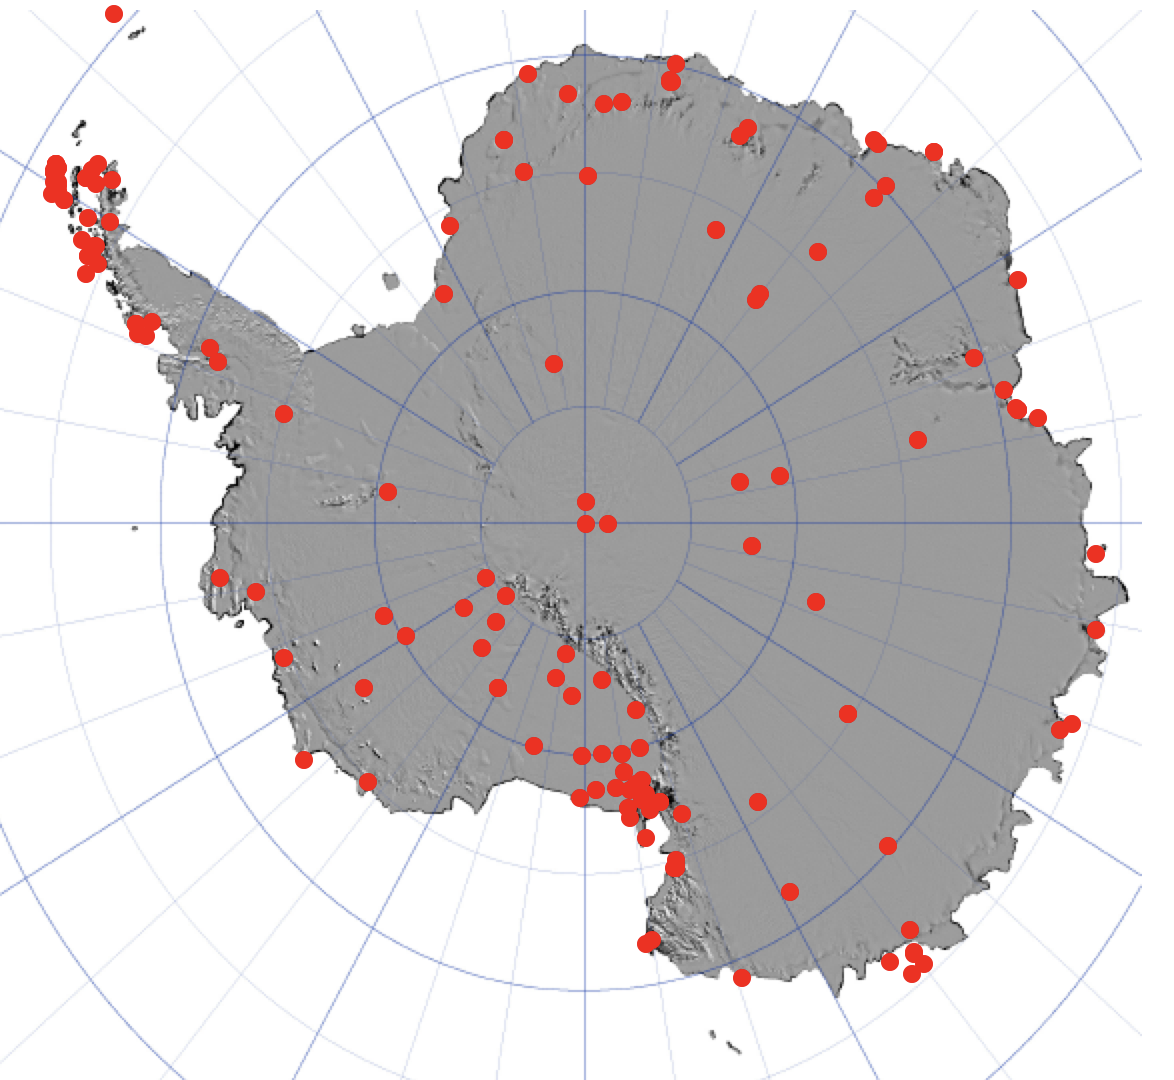
\includegraphics[width=\textwidth]{figures/BaseMap}
	\caption{A map of the recorded human activity on the continent of Antarctica during the ANITAIII flight.}
	\label{fig:BaseMap}
\end{figure}	
	
	
	\subsection{Event Clustering and Log Likelihood}
		Impulsive events that point back to a geographically isolated source location have the highest likelihood to be astrophysical in nature.  The metric that has been used in past ANITA experiments to determine the ``closeness'' of one event to another has been called the Log Likelihood, and is represented by the variable $L$.  This measurement must take into account both the pointing uncertainty of the instrument, as well as the constantly changing payload location.
		
		The pointing resolution of the interferometric mapping technique is a function of the SNR, and thus any clustering analysis must factor this into its calculation.  The pointing resolution as a function of SNR was found from analyzing self triggered WAIS pulses and their subsequent pointing to the 
		
		As ANITA transits past anthropogenic sources on the continent, the payload coordinate pointing towards that base changes with respect to cardinal North. In order to determine whether the likelihood that any particular event fell close to another, one must project the geographical location where the first event pointed to the continent into the field of view of the second event payload locations.  The opposite must be done as well, projecting the second event source location into the field of view of the first event payload location, as the two processes are not strictly invertible.
	\begin{equation}
		L = \sqrt{(\frac{\sqrt{(\Delta\phi_{AB})^2+(\Delta\phi_{BA})^2}}{{\sigma_{\phi}}})^2+(\frac{\sqrt{(\Delta\theta_{AB})^2+(\Delta\theta_{BA})^2}}{{\sigma_{\theta}}})^2}
	\end{equation}
	


	\subsection{Impulsive source clustering}
	
